\documentclass[onecolumn]{article}
\usepackage{url}
\usepackage{algorithmic}
\usepackage[a4paper]{geometry}
\usepackage{datetime}
\usepackage[margin=2em, font=small,labelfont=it]{caption}
\usepackage{graphicx}
\usepackage{mathpazo} % use palatino
\usepackage[scaled]{helvet} % helvetica
\usepackage{microtype}
\usepackage{amsmath}
\usepackage{subfigure}
% Letterspacing macros
\newcommand{\spacecaps}[1]{\textls[200]{\MakeUppercase{#1}}}
\newcommand{\spacesc}[1]{\textls[50]{\textsc{\MakeLowercase{#1}}}}

\title{\spacecaps{Lab report: SW01 }\\ \normalsize \spacesc{TSM\_AnTeDe} }

\author{Fabian Gröger\thanks{fabian.groeger@hslu.ch}\\Hochschule Luzern}
\date{\today}

\begin{document}
\maketitle

\begin{abstract}
Abstract goes here
\end{abstract}

\section{Introduction}
Introduction here.

\begin{align}
	\mathcal{L} = \frac{1}{n}\sum_n^{i=1} (Y_i - \hat{Y}_i)^2
\end{align}

\begin{figure}[t]
\centering
    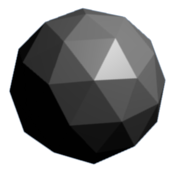
\includegraphics[width=.3\linewidth]{fig/flat.png}
\caption{\label{fig:demo-bad}
Caption}
\end{figure}

\begin{figure}[t]
\centering
\subfigure[Standard rendering]{\centering
    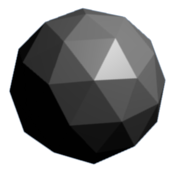
\includegraphics[width=.3\linewidth]{fig/flat.png}
        \label{fig:demo-standard}}
\subfigure[Fancy rendering]{\centering
    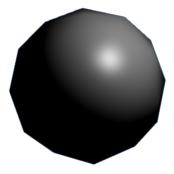
\includegraphics[width=.3\linewidth]{fig/smooth.png}
        \label{fig:demo-fancy}}
\caption{\label{fig:demo} 
Caption}
\end{figure}

\nocite{*}
\bibliographystyle{plain}
\bibliography{references}
\end{document}

